
\documentclass[sigconf]{acmart}

\usepackage{todonotes}
\usepackage{hyperref}

\usepackage{endfloat}
\renewcommand{\efloatseparator}{\mbox{}} % no new page between figures

\usepackage{booktabs} % For formal tables

\settopmatter{printacmref=false} % Removes citation information below abstract
\renewcommand\footnotetextcopyrightpermission[1]{} % removes footnote with conference information in first column
\pagestyle{plain} % removes running headers

\begin{document}
\title{Mapping Police Killing of Citizens in the United States}

\author{Jeramy Townsley}
\orcid{1234-5678-9012}
\affiliation{%
  \institution{IUPUI}
  \streetaddress{425 University Ave}
  \city{Indianapolis} 
  \state{Indiana} 
  \postcode{46202}
}
\email{jtownsle@indiana.edu}


\begin{abstract}
With the rise of camera phones that allows citizens to videotape law enforcement brutality against citizens, and the ability to immediately make those videos public through social media, there has been an increased awareness of police killings of citizens, and a number of systematic attempts to document these events, since there is no government database that has been shown to be credible on this issue. These events can be mapped at the county level (3,143 counties in the US are listed in the 2015 Census Tiger shapefiles) with the open source software QGIS.  Further, demographic and economic data gathered by the Census at the county level (5-year estimates as of 2015 with the American Community Survey) can be collected and tested against the police-killings data to determine if a regression model can be used to describe a significant pattern among these variables. 
\end{abstract}

\keywords{i523, hid347, police brutality, multivariate regression, gis mapping, census, zero-inflated models}

\maketitle

\section{Introduction}


\begin{figure}
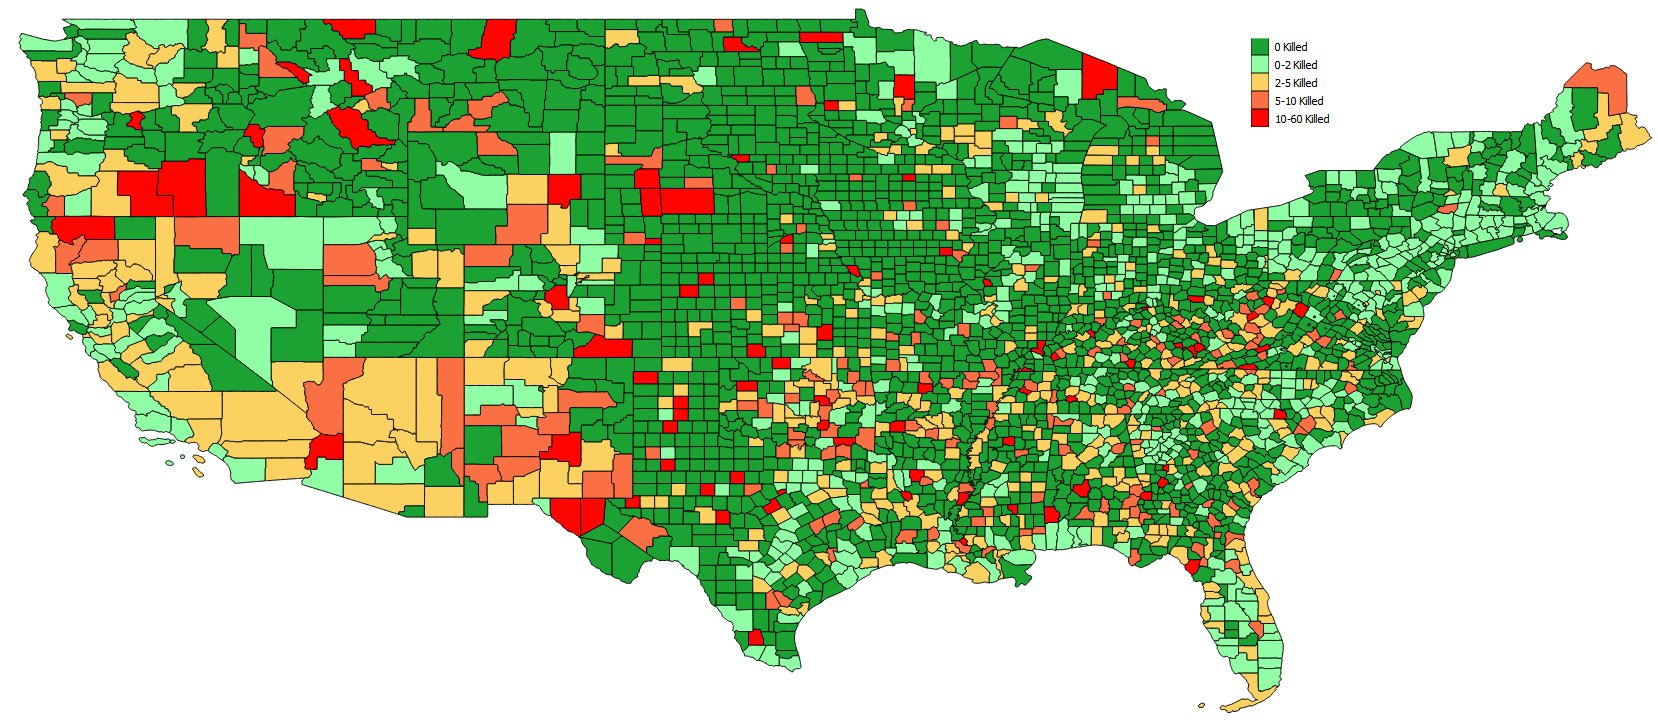
\includegraphics[width=1.0\textwidth]{images/figure1.jpg}
\caption{U.S. county-level map of residents killed by police, 2013-Oct 2017.  Data from Census and MappingPoliceViolence.org}
\end{figure}

\begin{figure}
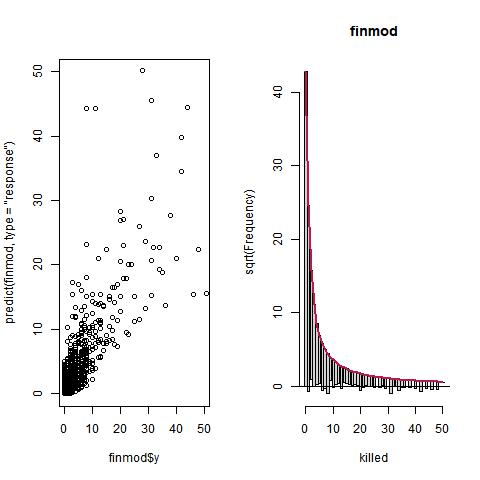
\includegraphics[width=1.0\textwidth]{images/figure2.jpg}
\caption{Plots of predicted versus observed, and rootogram of predicted, for the final regression model, negative binomial, three independent variables: population (log), employment and median income.}
\end{figure}

\begin{figure}
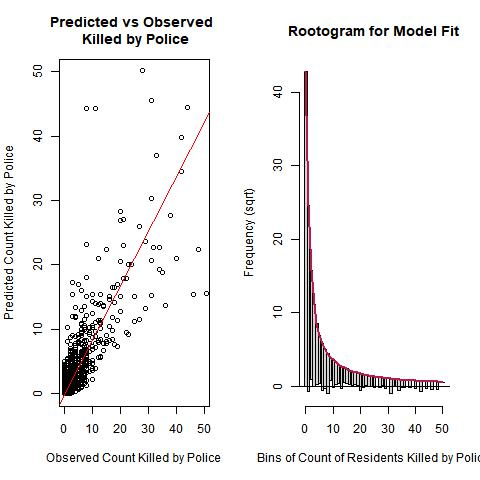
\includegraphics[width=1.0\textwidth]{images/figure3.jpg}
\caption{Regression diagnostics plots for the final model with three independent variables: population (log), employment and median income. Top: Residuals versus fitted and index.  Bottom: Quantile residuals and QQ Plot. }
\end{figure}


\section{Conclusion}
\bibliographystyle{ACM-Reference-Format}
\bibliography{report} 

\end{document}
